\section{Dynamic VMPP Algorithms}
\label{sec:vm-schedulers}

To illustrate the interest of \vmps, we implemented three dynamic VM
placement mechanisms: a centralized one based on the Entropy
proposal~\cite{Hermenier:2009:ECM:1508293.1508300}, a hierarchical one
based on Snooze~\cite{feller:ccgrid12}, and a fully-distributed one
based on DVMS~\cite{quesnel:cpe2012}.

\MS{We should differentiate more clearly between the complete VMPP
  system and the solver.}

These systems enable  the resolution  of violations in form of
overloaded nodes. A host is overloaded when the VMs try to consume
more than 100\% of the CPU capacity of the host. In such a case, a
resolution algorithm looks for an optimal viable configuration until
it reaches a predefined timeout. In all cases, we chose to use the
latest solver developed as part of the Entropy
framework~\cite{hermenier:cp11} as this resolution algorithm.
% Giving up consolidation optimality in favor of scalability, this
% algorithm provides a ``repair mode'' that enables the correction of VM
% requirement violations. The optimal solution is a new placement that
% satisfies the requirements of all VMs while minimizing the cost of the
% reconfiguration.
Once the timeout has been triggered, the algorithm returns the best
solution among the ones it finds and applies the associated
reconfiguration plan by invoking live migrations in the simulation
world.
%
% Although using the Entropy VMPP solver implies a modification from the
% original Snooze proposal, we highlight that our goal is to
%
% and thus we believe that such a modification is acceptable as it
% does not change the global behavior of Snooze

Simulating these three VMPP systems illustrates the capabilities of
\vmps. Moreover, by conducting such a comparison, we also investigate
the pros and cons of the three architecture models on which these
proposals rely on (\ie centralized, hierarchical and distributed).

In the remainder of this section, we first present an overview of the
three systems, showing, in particular, that the extended abstractions
for hosts (\texttt{XHost}), VMs (\texttt{XVM}) and the functions of
the \sg MSG API enabled us to develop them in a direct and natural
manner. We then present simulation results that, as a first, allow the
three approaches to be compared.

\subsection{Entropy-based Centralized Approach}
\label{subsec:entropy}
The centralized VM placement mechanism consists in one single \sg
process deployed on a service node. This process implements a simple loop that
iteratively checks the viability of the current configuration by
invoking seconds the aforementioned VMPP solver with a predefined
frequency.
% $p$ is defined as an input parameter of the simulation.

% \AL{Should we explain the issue right now or not if we add VMPP section}
% Indeed, during
% the computation and the application of a schedule, the algorithm does
% not enforce QoS properties anymore, and thus cannot react quickly to
% violations. Second, since the manipulation of VMs is costly, the time
% needed to apply a new schedule is particularly important: The longer
% the reconfiguration process is, the higher is the risk that the schedule may
% be outdated, due to the workload fluctuations, when it is eventually
% applied.
% \vmps enables researchers to investigate such concerns in-depth.

% As the Entropy proposal does not provide a specific mechanism for the
% collection of resource usage information but simply uses an external
% tool (namely ganglia), we had two different ways to implement the
% monitoring to process: either by implementing additional asynchronous
% transmissions as a real implementation of the necessary state updates
% would proceed or, in a much more lightweight manner,
We monitor the resource usage through direct accesses
% by the aforementioned process
to the states of the hosts and their respective VMs, while accounting
for communication overheads explicitly
% induced by communication in the ``real'' implementation, for
% instance, can be easily added as part of the lightweight
% simulation. We have implemented this lightweight variant for the
% monitoring
%
% Regarding fault tolerance, similarly to the Entropy proposal, our
% implementation does not provide any failover mechanism.
%
% as mentioned in Section \ref{subsec:traces-analysis},
We also monitor, for each iteration, whether the VMPP solver succeeds
or fails. In case of success, \vmps records the number of migrations
that have been performed, the time it took to apply the
reconfiguration and whether the application of the reconfiguration
plan led to new violations.

\subsection{Snooze-based Hierarchical Approach}
\label{subsec:snooze}
We now present Snooze~\cite{feller:ccgrid12} as a second case study of how
to implement and simulate advanced algorithms.
We present its architecture summarizing its main
characteristics from its original presentation~\cite{feller:ccgrid12} and
additional information  stemming from personal communications of the Snooze
developers and its implementation~\cite{snoozeweb,snoozedev14}.

\subsubsection{Architecture}
\label{sec:snoozeArchi}

Snooze harnesses a hierarchical architecture in order to support load
balancing and fault tolerance, cf.\ Fig.~\ref{fig:snoozearch}.

\begin{figure}[hbp]
  \begin{center}
  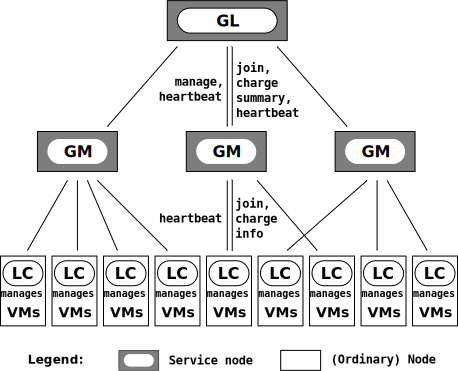
\includegraphics[width=.85\linewidth]{figures/snoozearch.pdf}
  \caption{Overview of Snooze's architecture}
  \label{fig:snoozearch}
\end{center}
\vspace*{-.3cm}
\end{figure}

At the
top of the hierarchy, a \emph{group leader (GL)} centralizes
information about the whole cluster using summary data about
\emph{group managers (GMs)} that constitute the intermediate layer of
the hierarchy. GMs manage a number of \emph{local controllers (LCs)}
that, in turn, manage the VMs assigned to nodes. The GL and the GMs
are deployed on service nodes while the LCs are executed on hosting
node.  During execution, higher-level components periodically send
heartbeats to lower-level ones; monitoring information, \eg about the
system load, is also sent periodically in the opposite direction. In
order to propagate information down the hierarchy, Snooze relies on
hardware support for multicast communication. Finally, a number of
replicated entry points allows clients to contact the GL, \eg in order
to submit new VMs for integration into the system.

\emph{Simulation using \vmps.~} The \texttt{XHOST}, \texttt{XVM} and
\texttt{SimulatorManager} classes have been harnessed to implement the
core architectural abstractions (\ie VM monitoring and manipulations),
the remaining concepts and algorithms of Snooze have been implemented
using Simgrid's primitives and standard Java mechanisms.
%
Communication between Snooze actors is implemented based on Simgrid's
primitives for, mainly asynchronous, event handling.
Hardware\-sup\-ported multicast communication that is used, \eg
to relay heartbeats, is implemented as a dedicated actor that manages
a state representing GL and GM heartbeat groups and relaying heartbeat
events.
%
Finally, our Snooze simulation uses, as its original counterpart, a
multi-threaded implementation (\ie based on multiple SG processes) in
order to optimize reactivity even for large groups of LCs (or GMs)
that have to be managed by one GM (or GL).

\subsubsection{Algorithms}
\label{sec:snoozeAlgs}

Apart from the handling of faults (described below), two types of
algorithms are of major importance for the administration of the
Snooze architecture: the algorithms that enable components to
dynamically enter the system and the algorithms that propagate info
between the components.

A GL is created, if it does not exist, by promotion of a GM that is
selected according to some leader election algorithm. When a GM joins
a cluster, it starts listening on a predefined channel for the
heartbeat of the GL and registers once it has received the
heartbeat. New LCs first also wait for the GL heartbeat, contact the
GL then in order to obtain a GM assignment, and finally register at
the GM assigned to them.

Two kinds of (load) information are passed within the system: the
periodic heartbeat message sent by the GL and the GMs; second,
periodic load information sent from LCs to their respective GMs and
summary load info sent by the GMs to the GL.

\subsubsection{Fault tolerance}

GLs, GMs and LCs may fail during the system execution. System
components identify that a node on the corresponding higher-level node
has failed (the GL in case of a GM, a GM in the case of an LC) in an
asynchronous fashion through the lack of heartbeat messages.

In the case of a GL failure, one of the GMs becomes the new GL, stops
its GM activities and prevents the LCs it manages so that they can
start rejoining the system. If a GM fails, the GL and the LCs it has
managed will become aware of it based on the lack of heartbeats,
update its data structures and, for the LCs, rejoin the system. If an
LC fails, its GM will finally learn of it due to the missing heartbeat
and charge information of the LC. The GM will then remove the LC from
its data structures.


% \subsubsection{Variants}
% \label{sec:snoozeVariants}

% Our simulation framework facilitates the simulation of variants of
% placement algorithms. In the following, we present three non-trivial
% variants that we have implemented and explored: a variant of the
% assignment algorithm of LCs to GMs, periodic vs.\ reactive scheduling,
% and a variant of the algorithms of how GMs and LCs join the system.


% \paragraph{Assignment of LCs to GMs}

% LCs are assigned to GMs by the GL as part of the LC join protocol. In
% Snooze's native implementation LCs are assigned in a round-robin
% fashion to the known GMs. If GMs join (and leave) the system at the
% same time as LCs, a round-robin strategy at join time, however, does
% not ensure an even distribution. This may happen, for instance at
% startup time of the system, when new GMs and LCs enter the system, or
% in case of failures, which trigger GM and LC joins. In order to
% evaluate the imbalance resulting from a round-robin strategy (as well
% as others) we have implemented the LC assignment protocol in a modular
% fashion and applied it in diverse highly-dynamic settings in which GMs
% and LCs enter the system at the same time. Furthermore, we have
% implemented a best-fit strategy that assigns LCs to GMs with minimal
% load or to GMs with the smallest number of assigned LCs (if several
% GMs with minimal load exist). The best-fit strategy can significantly
% improve the scheduling characteristics of hierarchical placement
% algorithms as shown by the experimental data presented in
% Sec.~\ref{sec:snoozeVariantsEval}. Furthermore, it should always be
% at least as good as the round-robin strategy (the corresponding proof
% is left to future work).


% \paragraph{Periodic vs.\ reactive scheduling}

% Snooze~\cite{feller:ccgrid12} schedules VMs in a periodic fashion:
% after a fixed time period a GM calls the scheduler in order to resolve
% resource conflicts among the LCs it manages. The information whether a
% resource conflict has to be handled is taken based on the summary
% information that is periodically sent by the LCs to the GM.

% We have provided an alternative, reactive, strategy to scheduling: as
% soon as they occur, LCs avert their GMs of resource conflicts; the GMs
% then initiate scheduling. Implementing this reactive scheme can be
% done using our framework in two manners: either by implementing
% additional asynchronous transmissions as a real implementation of the
% necessary state updates would proceed or, in a much more lightweight
% manner, through direct accesses by the GMs to the states of their
% respective LCs. While the latter does not mimic a real implementation
% closely, it can be harnessed to yield a valid simulation: delays
% induced by communication in the ``real'' implementation, for instance,
% can be easily added as part of the lightweight simulation. We have
% implemented this lightweight variant of reactive scheduling.


% \paragraph{Variants of the join algorithms}

% The join algorithms, see Sec.~\ref{sec:snoozeAlgs}, are crucial to the
% correctness of Snooze for two main reasons: (i) they have to be
% efficient because they can easily form a bottleneck if large numbers
% of LCs (GMs) have to be registered at a GM (LC); (ii) they are
% multi-phase protocols whose correctness especially in the presence of
% faults is difficult to ensure.

% In order to investigate the corresponding trade-offs, we have used our
% framework to implement join algorithms that may be interrupted at any
% time, repeat the the on-going phase a number of times before
% reinitiating, if necessary, the entire protocol. Furthermore, the join
% protocol is parameterized, \eg, in the number of threads used to
% handle registration requests.

% Finally, our framework has enabled us to test another aspect of
% Snooze's join algorithm as presented by
% Feller~\etal.~\cite{feller:ccgrid12},
% \MS[MS]{If we succeed to perform the experiment comparing both
%   approach, this paragraph should be highlighted.}
% a strategy we call the GM rejoin
% strategy (GRJ): all GMs should rejoin if a new GM enters the
% system. While GRJ supports a form of load balancing (because all LCs
% are reassigned to the new set of GMs), our simulation has shown that
% this strategy significantly increases the time necessary for
% registering GMs and LCs compared to a simpler strategy that does not
% modify existing GMs in case a new GM enters the system. This handicap
% is particularly pronounced if joins of GMs may be interrupted due to
% faults. Concretely, experiments involving 20 GMs and 200 LCs have
% shown that this strategy often multiplies the time necessary to join
% all 220 components by 10 or more compared to the simple join
% strategy. While the qualitative result that the more complex strategy
% presented in the paper results in a more time-consuming join process
% is not very surprising, the extent of the resulting degradation was
% surprising.



%%% Local Variables:
%%% mode: latex
%%% TeX-master: "main"
%%% End:


\subsection{DVMS-based Distributed Approach}
\label{subsec:dvms}
% TODO Not adressed
%\AL[AL]{Check who write that part, If Flavien did it, then add him as
%  an author}
DVMS~\cite{quesnel:cpe2012} (Distributed Virtual Machine
Scheduler) is a framework that schedules VMs cooperatively and dynamically in
large-scale distributed systems.

\subsubsection{Overview and Definitions}
From a software point of view, the nodes are organized following a ring
topology.

A scheduling procedure is started as soon
as an event occurs on the infrastructure.

Each event is associated with a partition.  A partition is composed of all the
nodes that are reserved for the resolution of a specific event.
%
Partitioning the infrastructure is mandatory to avoid conflicts between several
schedulers that could manipulate the same nodes or VMs when they apply their
reconfiguration plans.

Each partition includes two special nodes, the initiator and the leader.
The initiator of a partition is the node that
initially produced the event associated with this partition.
The leader of a partition is the node that leads the scheduling computations
aiming at solving the event associated with this partition; the leader of
the partition is likely to change during the processing of the event.


\subsubsection{The Problem Solving Procedure}

The problem solving procedure is initiated when a node
N\(_{\textit{i}}\) observes that there is a problem, for instance when its
resources are overused (see Figure~\ref{fig:dvms_pte}); it then generates an
event and reserves itself to process this event (see
Figure~\ref{fig:dvms_pte_1}).  After that, it forwards this event to its
neighbor on the ring, node N\(_{\textit{i+1}}\).

If N\(_{\textit{i+1}}\) is already involved in another partition, it directly
forwards the event to node N\(_{\textit{i+2}}\); otherwise, N\(_{\textit{i+1}}\)
joins the new partition (see Figure~\ref{fig:dvms_pte_2}) and checks that the
event is still valid.  If the event is not valid anymore (for instance because
the virtual machines demands for resources fluctuated), N\(_{\textit{i+1}}\)
cancels the reservations to destroy the partition and thus allow the nodes that
composed it to take part to other problem solving procedures.
%
On the contrary, if the event is still valid, N\(_{\textit{i+1}}\) notifies all
the nodes inside the partition that it is the new leader; in return, it receives
information regarding (i)~the capacities of each node and (ii)~the resources
consumed by the virtual machines hosted on each node.  It then starts a
scheduling computation; if no solution is found, the event is then forwarded to
node N\(_{\textit{i+2}}\).

N\(_{\textit{i+2}}\) repeats the same operations, that is to say: self-reservation
(if it is free, see Figure~\ref{fig:dvms_pte_3}), event validity check, leader
change notification, monitoring of VMs and nodes inside the partition,
scheduling computation.  If N\(_{\textit{i+2}}\) finds a solution, it applies the
corresponding reconfiguration plan that solves the event; it then cancels
reservations to destroy the partition and thus allow the nodes that composed it
to take part to other problem solving procedures.

Note that, if N\(_{\textit{i+2}}\) did not find a solution, the partition would
have grown until a solution was found or the even had traversed the whole ring.
In the latter case, the problem would be considered as unsolvable and the
partition would be destroyed.

The progressing increase in size of the partition aims at adapting it to the
complexity of the problem to solve.
This approach enables to consider as few nodes as possible, thus accelerating
the scheduling computations to solve the event as quickly as possible.

\begin{figure}[h]
\subfigure[]{
\includegraphics[width=3.8cm]{./figures/fig-24.pdf}
\label{fig:dvms_pte_1}}
%
\subfigure[]{
\includegraphics[width=3.8cm]{./figures/fig-25.pdf}
\label{fig:dvms_pte_2}}
%
\subfigure[]{
\includegraphics[width=3.8cm]{./figures/fig-26.pdf}
\label{fig:dvms_pte_3}}
%
\subfigure[Legend]{
\includegraphics[width=3.8cm]{./figures/fig-27.pdf}
\label{fig:dvms_pte_4}}
%
\caption{Processing two events simultaneously\label{fig:dvms_pte}}
\end{figure}


\subsubsection{Fault-tolerance}

The original implementation of DVMS was not fault-tolerant.


\paragraph{Repairing the Ring.}

Making DVMS fault-tolerant implied first to make the ring fault-tolerant.
Previously, if a node \emph{N\(_{\textit{i}}\)} crashed, an event passing through
node \emph{N\(_{\textit{i-1}}\)} could not reach node \emph{N\(_{\textit{i+1}}\)}.

To preserve the integrity of the ring, we used the algorithms
designed for Chord~\cite{stoica:2001:sigcomm01}.
%
The main idea is to let each node know not only its neighbor, but also its
2\(^{\textit{1}}\) successor, its 2\(^{\textit{2}}\) successor, and so on until the
2\(^{\textit{i}}\) successor, \emph{i} being specified by the administrator;
%
when some part of the ring crashes, network communications can still be
performed by passing through a known alive successor.


\paragraph{Destroying a Partition If One of Its Node Fails.}

Having a fault-tolerant ring was not enough; it was also necessary to make the
problem solving procedure fault-tolerant.

Previously, if the leader of a partition crashed, the problem identified by the
initiator would never be solved; moreover, the nodes of this partition would
remain reserved indefinitely and would not be able to take part to other problem
solving procedures.

To avoid these issues, DVMS now relies on a timeout.  Each node involved in a
partition periodically checks whether the state of its partition changed
recently (for instance, a new node joined the partition).
%
If the state does not change anymore, it probably means that the problem solving
procedure is stuck (maybe because the leader crashed).
%
In this case, each node decides to leave the partition and becomes free to take
part to other problem solving procedures.




%%% Local Variables:
%%% mode: latex
%%% TeX-master: "main"
%%% End:
